\documentclass{article}
\usepackage[utf8]{inputenc}
\usepackage{geometry}
\usepackage{amsmath}
\usepackage{graphicx}
\usepackage{enumitem}
\usepackage{float}
\usepackage{hyperref}

    %\usepackage{showframe} %This line can be used to clearly show the new margins

    \newgeometry{vmargin={15mm}, hmargin={20mm,20mm}}

\title{Homework 1\\
    \large Advanced Machine Learning \\
    Spring 2019\\
    Instructor : Anna Choromanska}

\author{Vishwali Mhasawade (Net ID : vvm248)}
\date{February 2019}

\begin{document}

\maketitle

\section{Problem 1}
Considering a regression problem. Feature Space is denoted by $\mathcal X$ and interval space as $\mathcal Y$. Constructing a mapping $f : \mathcal X \rightarrow \mathcal Y$ to predict the label $y \in \mathcal Y$ for the feature $x \in \mathcal X$. Mapping is defined by a polynomial of degree $d$:
    \begin{equation}
        f(x;\theta) = \theta _0 + \theta_ 1 x + \theta_2 x^2 + .... + \theta_d x^d
    \end{equation}
\\
The task is to explore the setting of $d$ such that the parameter vector $\theta = \{ \theta_1, \theta_2,...,\theta_d \}$ minimize the loss function\\
\begin{equation}
    L(\theta) = \frac{1}{2N} \sum _{i=1} ^{N} (y_i - f(x_i;\theta)^2)).
\end{equation}
\subsection{Solution}
The dataset is split into two-halves (train and test data). 10-Fold cross-validation is performed to find the optimal $d$ setting that minimizes the loss. The training error ($tr _{error}$) and test error ($ts_{error}$) is calculated for $d \in \{0,1,2,...,13\}$. The errors in each fold of cross-validation are averaged to obtain the $tr_{error}$ and $ts_{error}$ respectively for each setting of $d$.\\
\\
With increasing $d$, the $tr_{error}$ decreases however there is an optimal $d$ for which $ts_{error}$ is minimum. The reason for this behavior is that if a polynomial of degree $k$ fits the training data, then every polynomial with degree $d > k$ will also fit the data. The coefficients $\{ \theta_{k+1}, \theta_{k+2}, .... \}$ become infinitesimally small to fit the data that is also fit by $k$ order polynomial. Thus, finding the best setting of the polynomial is not possible by just considering the training data. The test data obtained by splitting the original data into two-halves will be used for finding the optimal $d$. Since the parameter vector $\theta = \{ \theta_1, \theta_2,...,\theta_d \}$ is obtained from the training data, the same argument about the polynomial fit does not apply to the test data. There exists a value of $d$ for which the $ts_{error}$ is minimum and this is the value of $d$ chosen.

\subsubsection{Modeling the problem as a transformed linear regression}
The data ($data1.mat$) consists of rows corresponding to a data point ($x,y$) where $x$ is the feature (\textit{1-dimensional}) and $y$ is the corresponding label. To model this data as a linear regression, we need to transform it into another space. This transformation is represented as $\phi(x) = [ x^0 , x^1, x^2, .... , x^d ]$. After transforming the data, this represents a linear regression. The transformed model is \\
$y = \theta_0 \phi_0 (x) + \theta_1 \phi_1 (x) + ... + \theta_d \phi_d (x)$.

\[
\phi (X) = 
\begin{bmatrix}
x_1 ^ 0 & x_1 ^1 & x_1 ^2 & .... & x_1 ^d \\
x_2 ^ 0 & x_2 ^1 & x_2 ^2 & .... & x_2 ^d \\
.        & .     &        &      &        \\
.        & .     &        &      &        \\
.        & .     &        &      &        \\

x_N ^ 0 & x_N ^1 & x_N ^2 & ....  & x_N ^d 
\end{bmatrix}
\]
\\
Let $w = \{ \theta_1, \theta_2,...,\theta_d \} $. The closed from solution is \\
\\
\begin{equation}
    W = \big(\phi(X)^T \phi(X)\big) ^{-1} \phi(X) ^T Y 
    \label{w}
\end{equation}
The value of $W$ is calculated from equation \ref{w}.\\
\begin{figure}
    \centering
    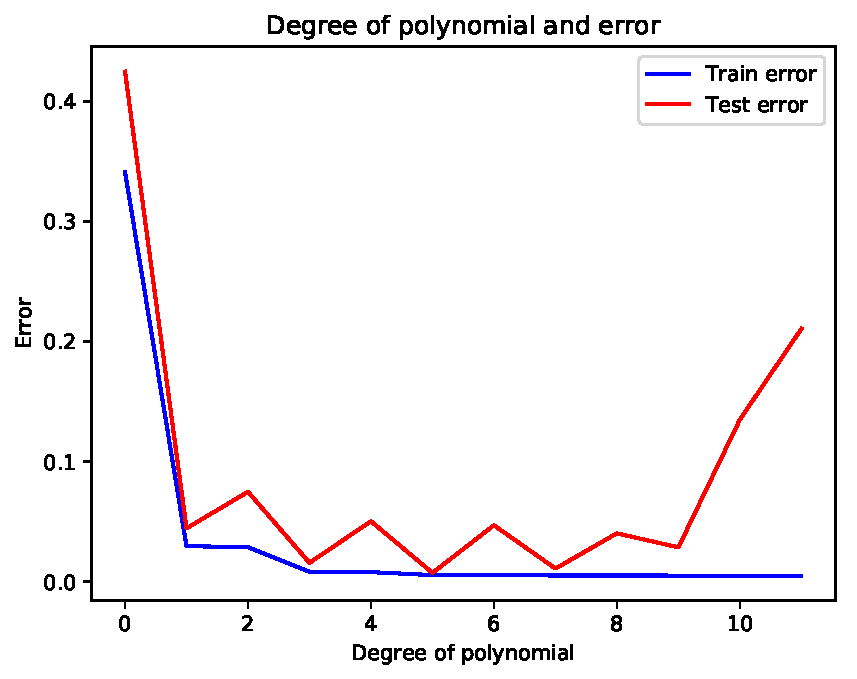
\includegraphics[scale = 0.9]{combined.pdf}
    \caption{Train and test error as a function of degree of polynomial $d$.}
 \label{fig:combined_error}
 \end{figure}

\\
Figure \ref{fig:combined_error} represents the training and test error as a function of the order of the polynomial $d$. As mentioned before the training error $tr_{error}$ continues to decrease with increasing order of the polynomial $k$. However, the test error $ts_{error}$ is the minimum for the value of $k = 5$. This elaborates the idea that a polynomial of degree \textbf {5} fits the training data well as well as generalizes on the test data. For $d > 5$, the training error $tr_{error}$ decreases but the test error $ts_{error}$ goes up and hence the search for $d$ is stopped beyond once $ts_{error}(k) > ts_{error}(5)$.

\begin{figure}
\centering
\begin{minipage}{.56\textwidth}
  \centering
  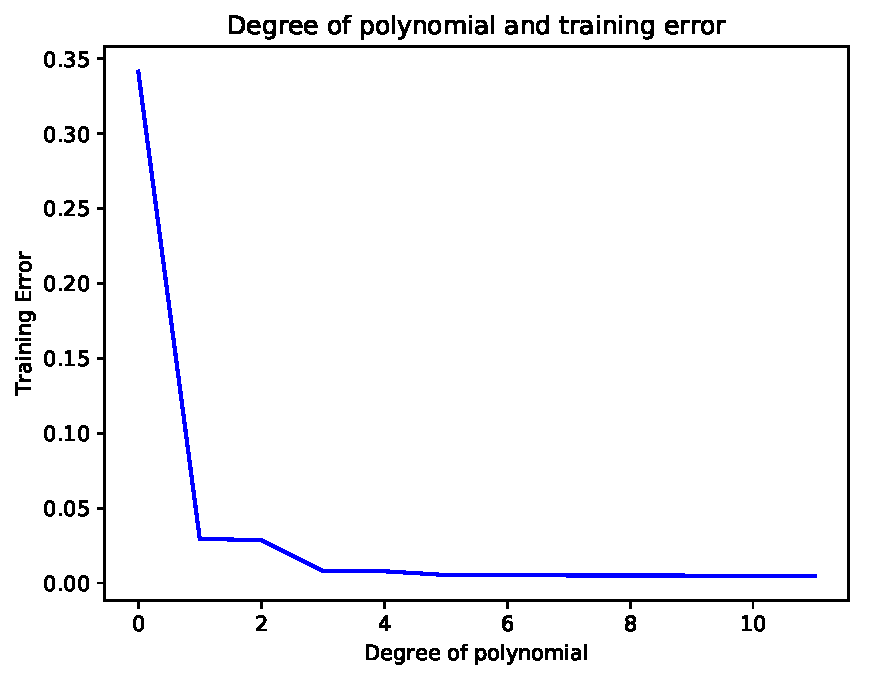
\includegraphics[scale = 0.5]{training_error.pdf}
  %\caption*{(i)}
  \label{fig:demo}
\end{minipage}%
\begin{minipage}{.6\textwidth}
  \centering
  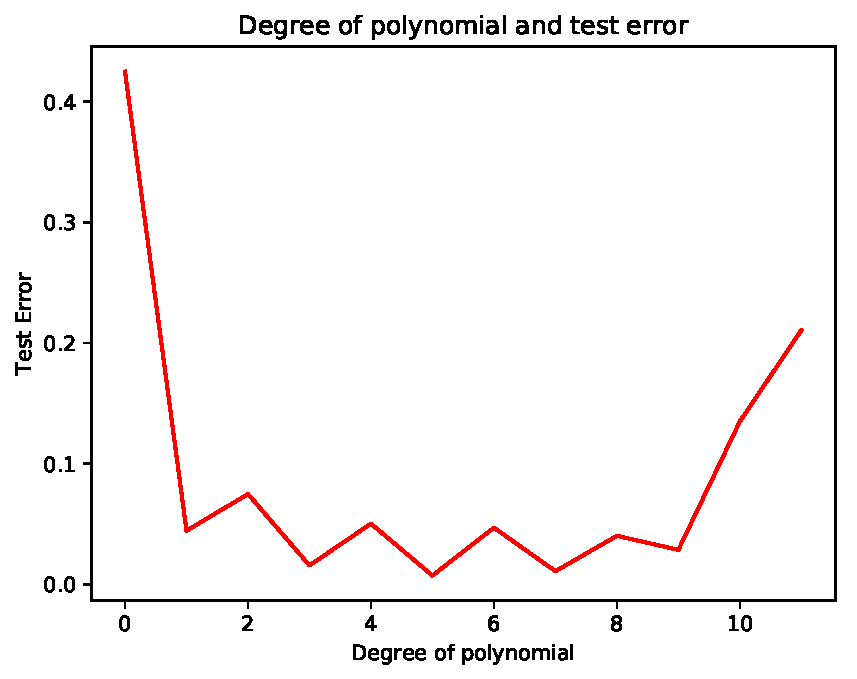
\includegraphics[trim = 10cm 0cm 0cm 0cm,scale=0.5]{test_error.pdf}
  %\caption*{(ii)}
  \label{fig:model}
  
\end{minipage}
\vspace{-0.425cm}
\caption{The left figure demonstrates the training error as a function of the degree of the polynomial. The right figure demonstrates the test error as a degree of the polynomial. }
\label{fig:model+demo}
\end{figure}


\section{Problem 2}
Consider a binary classification problem. Implement a linear logistic regression. Find a parameter vector $\theta$ for the classification function
\begin{equation}
    f(x;\theta) = (1 + exp(-\theta ^{T} x))^{-1}
\end{equation}
that minimizes the empirical risk given as 
\begin{equation}
\label{eq:loss}
    L(\theta) = \frac{1}{N}\sum_{i=1}^{N}(y_i -1 )log(1-f(x_i;\theta))- y_i log(f(x_1;\theta))
\end{equation}

\subsection{Solution}
The derivation is as follows:
\\
The gradient of the empirical risk with respect to the parameters $\theta$ is calculated:\\
\begin{equation}
    L(\theta) = \frac{-1}{N}\sum_{i=1}^{N}(1-y_i )log(1-f(x_i;\theta)) + y_i log(f(x_1;\theta))
\end{equation}

\begin{equation}
        \frac{\partial L(\theta)}{\partial \theta_{j}} = \frac{-1}{N}\sum_{i=1}^{N} \frac{\partial }{\partial \theta_j}(1-y_i )log(1-f(x_i;\theta)) + \frac{\partial }{\partial \theta_j}y_i log(f(x_i;\theta)) \\
\end{equation}
We consider the derivative for a single example which leads to SGD (Stochastic Gradient Descent).
\begin{equation} \label{eq:deriv}
\begin{split}
    \frac{\partial L(\theta)}{\partial \theta_{j}} &= -\Big(y \frac{1}{f(x;\theta)} - (1-y) \frac{1}{1-f(x;\theta)}\Big) \frac {\partial}{\partial \theta_j}f(x;\theta)\\
    &= -\Big(y \frac{1}{f(x;\theta)} - (1-y) \frac{1}{1-f(x;\theta)}\Big)f(x;\theta)(1-f(x;\theta)) \frac {\partial}{\partial \theta_j}f(x;\theta)\\
    &= -\Big(y(1- f(x;\theta)) - (1-y) (f(x;\theta))\Big)\frac{\partial}{\partial \theta_j}(\theta^{T}x)\\
    &= \big(f(x,\theta)-y\big)x_j
\end{split}
\end{equation}
The parameter update rule is as follows:
\begin{equation}
\label{eq:update}
    \theta \mathrel{-}= lr * X^{T}(f(X;\theta)-Y)
\end{equation}
where $X$ is the input feature matrix, $Y$ is the label vector and $\theta$ is the parameter vector. Equation \ref{eq:update} represents the parameter update rule in the vector notation. 
\begin{figure}[H]
    \centering
    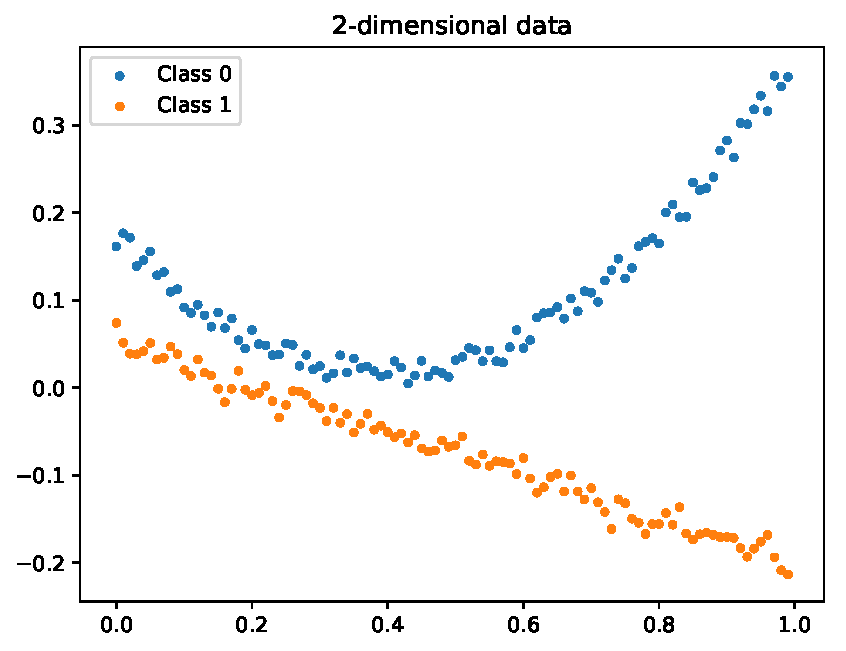
\includegraphics[trim = 0cm 0cm 0cm 0cm,scale = 0.75]{input_data.pdf}
    \caption{The data is linearly separable. The two classes are represented by the two colors}
 \label{fig:input_dta}
 \end{figure}
 
\begin{figure}[H]
    \centering
    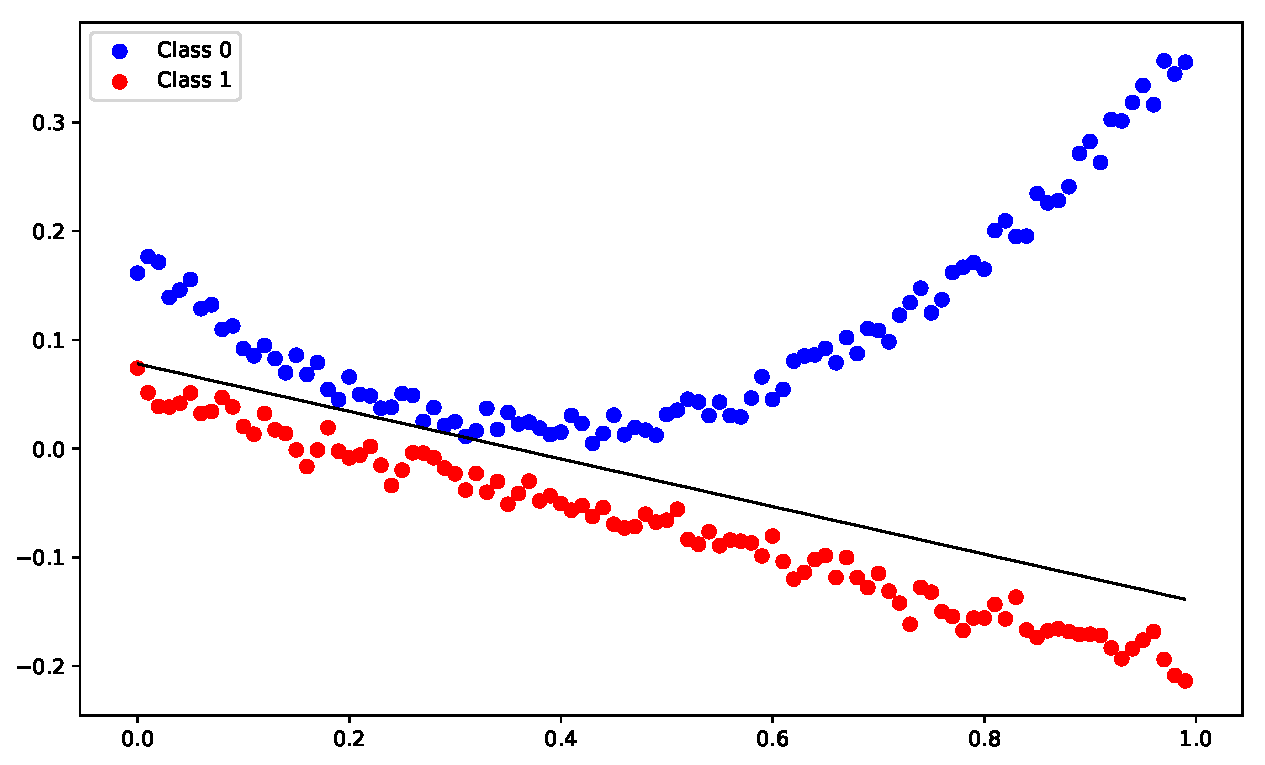
\includegraphics[trim = 0cm 0cm 0cm 0cm,scale = 0.7]{decision.pdf}
    \caption{Linear decision boundary}
 \label{fig:decision_bound}
\end{figure}

\begin{figure}[H]
    \centering
    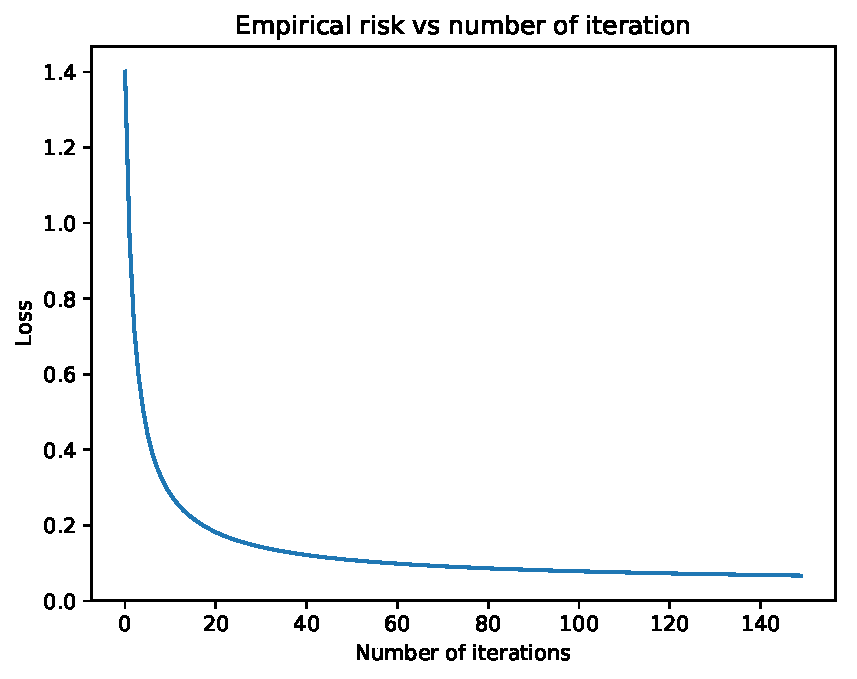
\includegraphics[trim = 0cm 0cm 0cm 0cm,scale = 0.8]{Risk_time.pdf}
    \caption{Empiricial risk for each iteration}
 \label{fig:risk}
\end{figure}

The data is linearly separable as show in Figure \ref{fig:input_dta}. The \textit{blue} and \textit{orange} represent the two classes \textit{Class 0} and \textit{Class 1} respectively. The linear decision boundary of the linear logistic regression is found by optimizing the parameters using the update rule from equation \ref{eq:update}. This decision boundary is shown in Figure \ref{fig:decision_bound}.\\
\\
The empirical risk given by equation \ref{eq:loss} decreases over time and when the parameter learning process finally converges. Since the empirical risk is a convex function in $\theta$, the minima can be found by finding the gradients till the process converges. This is derived in equation \ref{eq:deriv}.  The empirical risk vs number of iterations is shown in Figure \ref{fig:risk}.





\section{Problem 3}
Consider two ways of generalizing the concept of a linear discriminant function from two classes to $K$ classes.
\begin{enumerate}
\item Use $(K-1)$ linear discriminant functions $y_k$, where $k = \{1,2,3,...,K-1\}$, such that $y_k(x) > 0$ for inputs $x$ in class $C_k$ and $y_k(x) < 0$ for inputs not in class $C_k$.

\item Use one discriminant function $y_{jk}(x)$ for each possible pair of classes $C_j$ and $C_k$ such that $y_{jk}(x)> 0$ for all patterns in class $C_j$ and $y_{jk}(x) < 0$ for patterns in class $C_k$ (for $K$ classes this gives $K(K-1)/2$ discriminant functions).  
\end{enumerate}
Show on a simple example in two dimensions fir $K=3$ that both approaches can lead to ambiguous regions of \textit{x}-space.

\subsection{Solution}
The possible discriminant functions for $K$ class classification is represented below. Since, $K=3$, 3 regions/classes are assumed. The possible discriminant functions are represented by the discriminant line.
\subsubsection{Case 1}
2 linear discriminant functions ($K-1$) for $K=3$.
\begin{figure}[htpb]
    \centering
    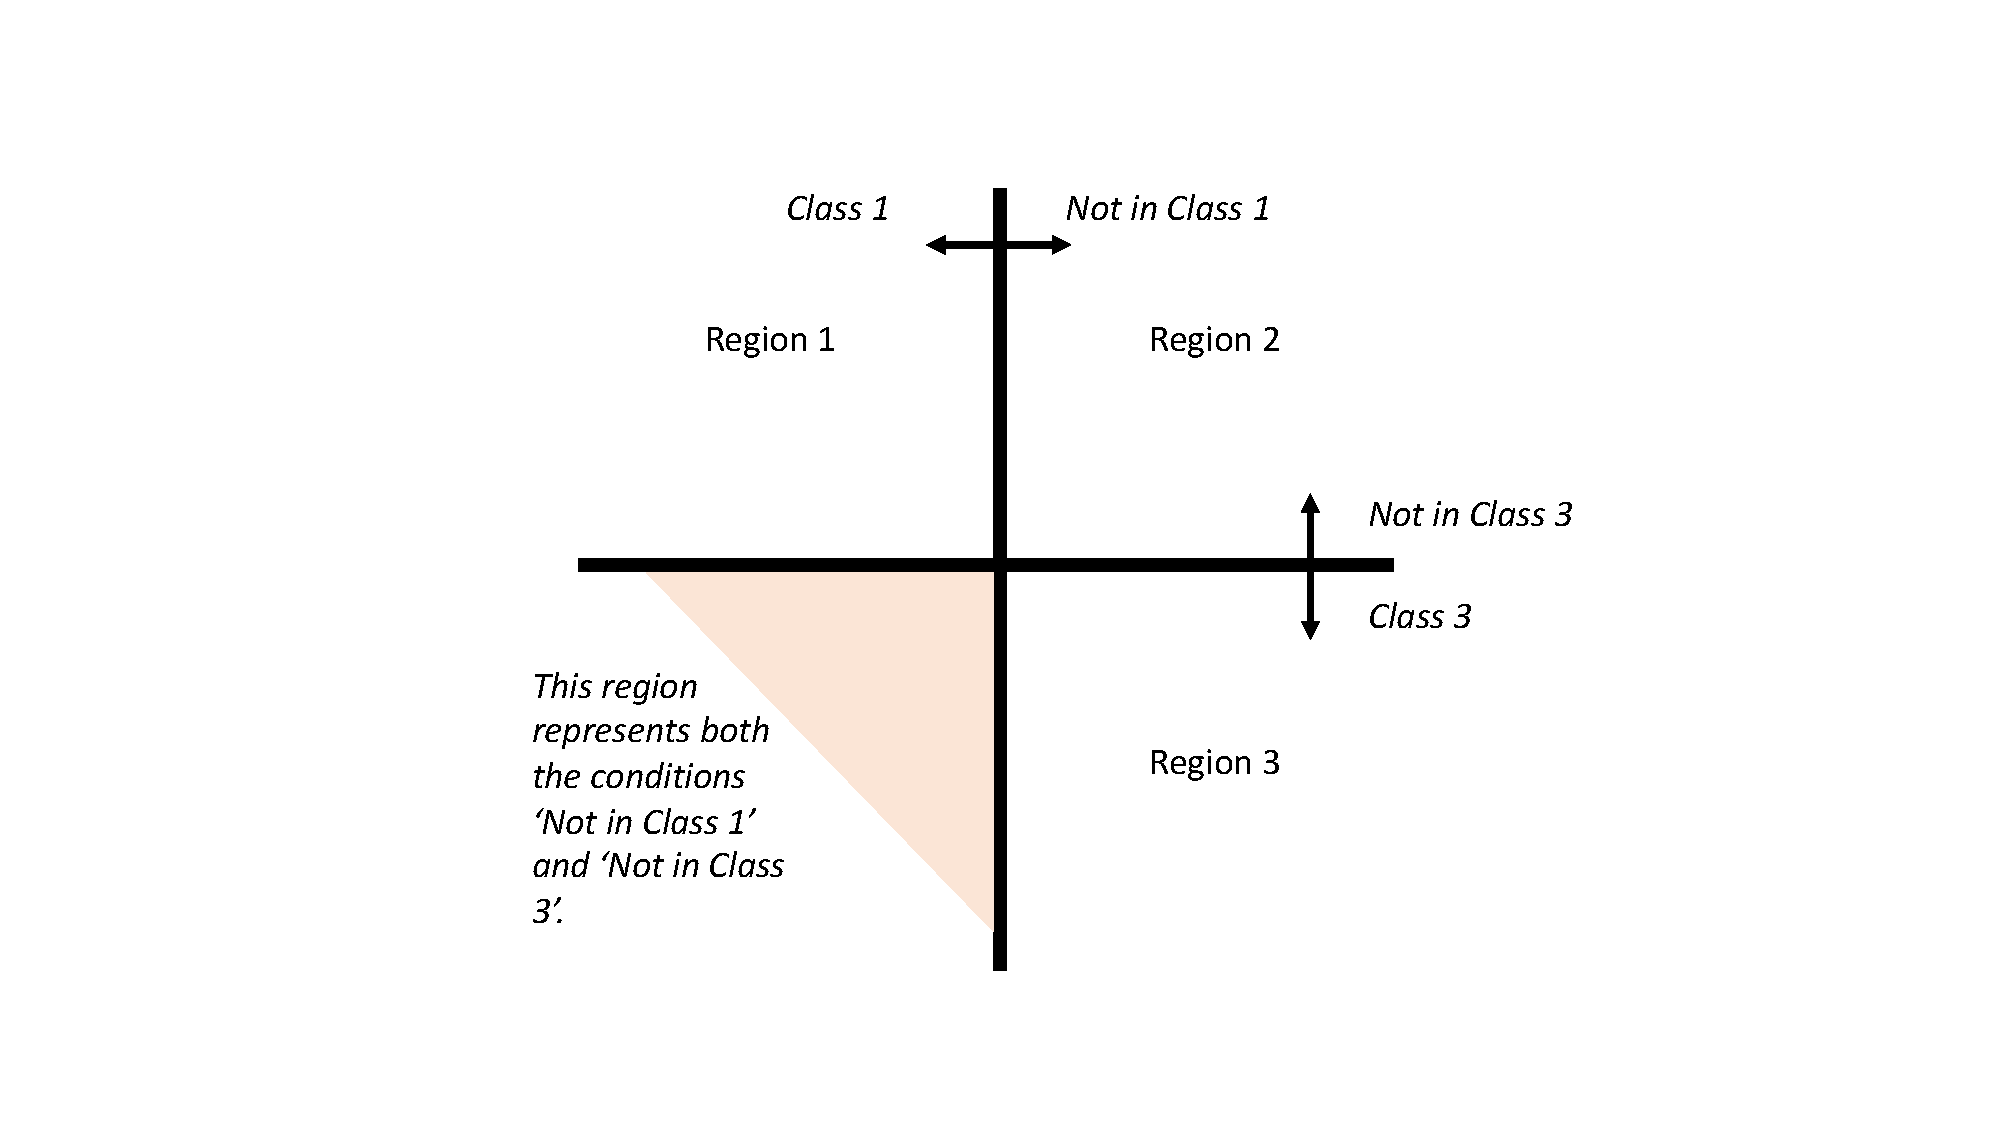
\includegraphics[scale = 0.5]{first_condition.pdf}
    \caption{2 ($K-1$) linear discriminant functions.}
 \label{fig:case1}
 \end{figure}
\\
There is an ambiguity to label patterns in the colored region since it represents two conditions mentioned in Figure \ref{fig:case1}.


\subsubsection{Case 2}
3 linear discriminant functions $K(K-1)/2$ for $K=3$.
\begin{figure}[H]
    \centering
    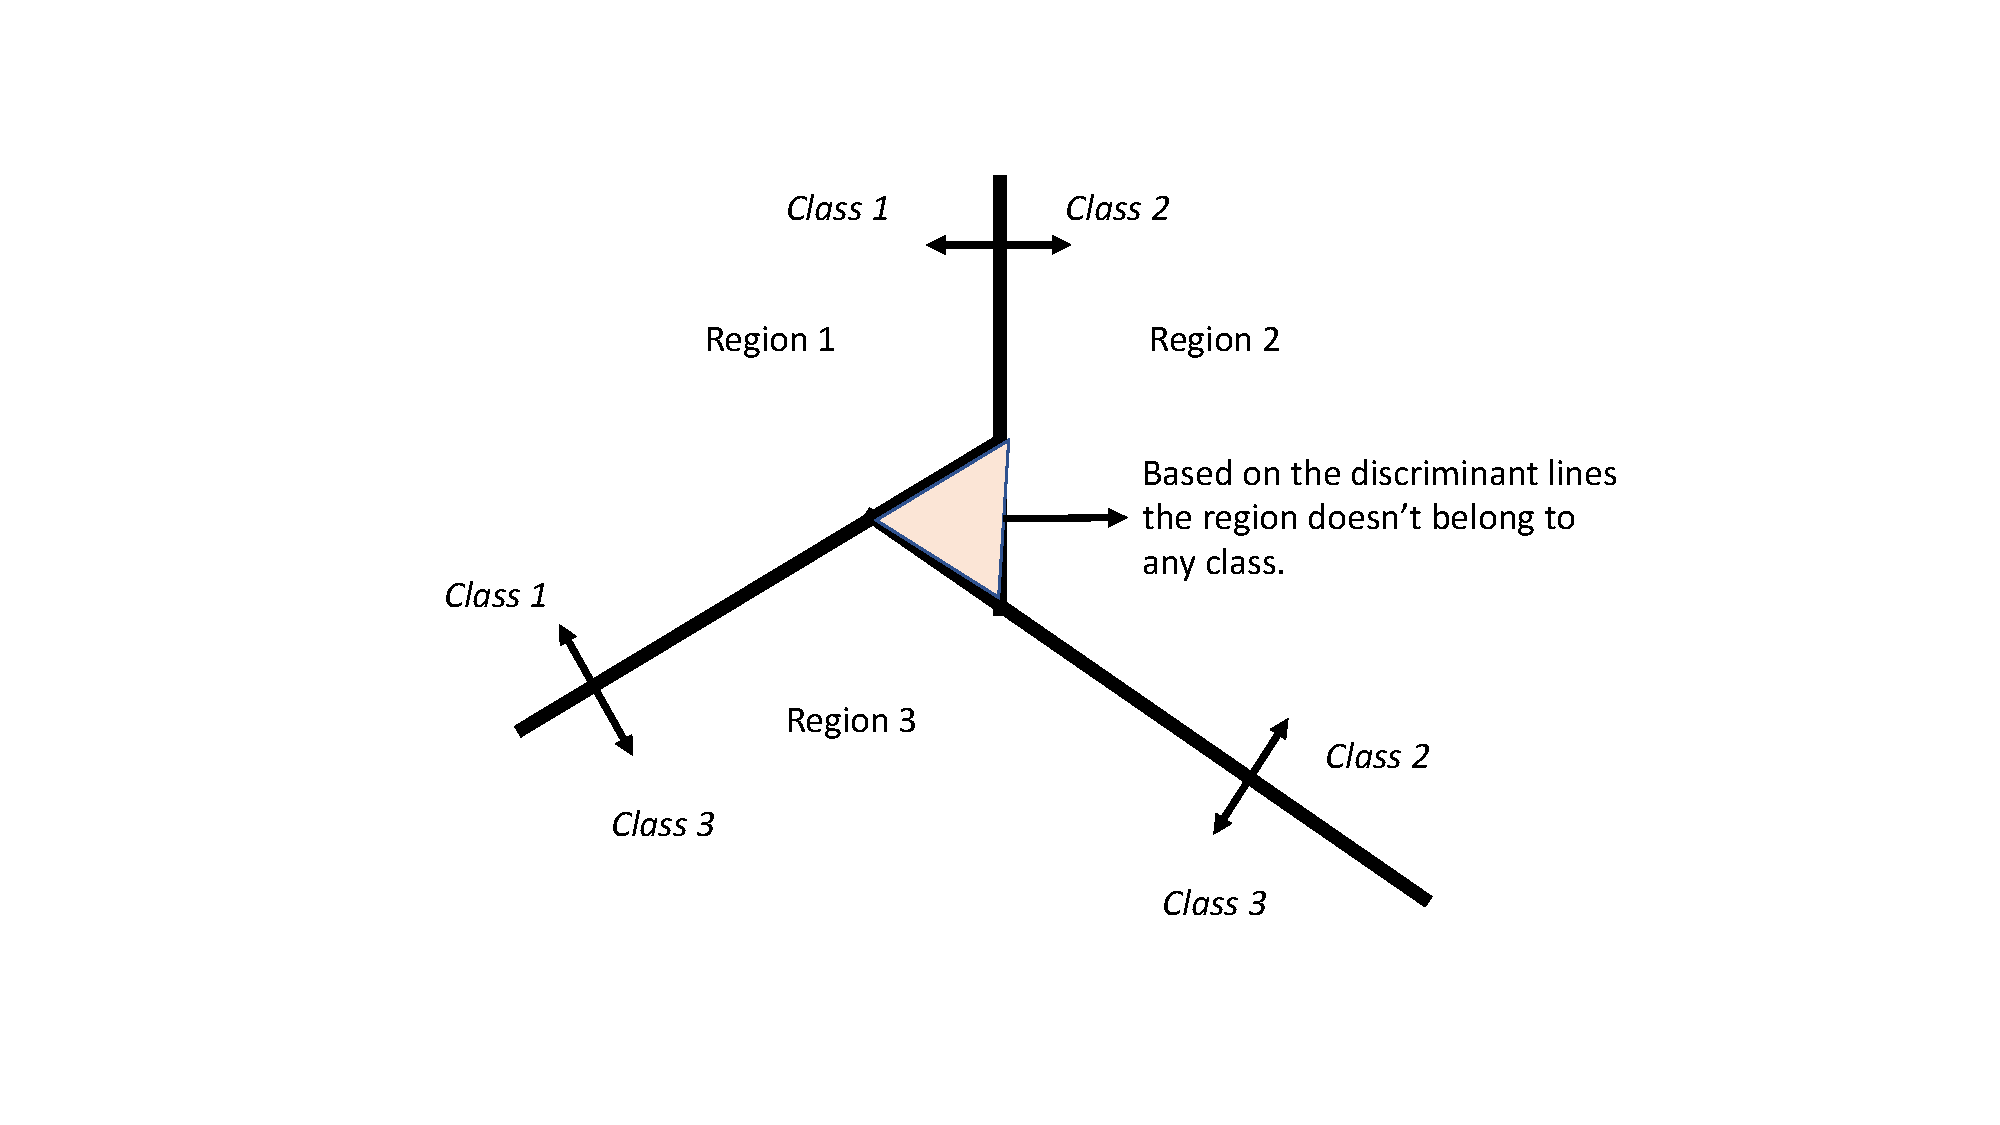
\includegraphics[trim = 0cm 0cm 0cm 0cm,scale = 0.5]{second_condition.pdf}
    \caption{3 : ($K(K-1)/2$) linear discriminant functions.}
 \label{fig:case2}
 \end{figure}
The colored region does not belong to any of the classes if we consider a discriminant function for every pair of classes as represented in Figure \ref{fig:case2}.\\
\\
Thus, these two cases represent that the approaches can lead to ambiguous regions of the two-dimensional space.

% \footnote{Code can be found at: \url{https://github.com/mvishwali28}}

\end{document}